% Generated from tex/chapters/ch04/09_ソフトウェア構築ツール.tex for the SWEBOK structure tree
\subsubsection{プロファイリング、性能分析、スライシングツール}

プロファイリングツールは、実行中のプログラムを監視し、各文や関数がどれだけ実行されたか、どれだけ時間を使ったかを記録する。これにより、性能上のホットスポットを見つけられる。

プログラムスライシングは、ある変数や処理結果に影響し得る文の集合を計算する技法である。デバッグ、プログラム理解、最適化分析に役立つ。静的解析や動的解析を使ってスライスを求めるツールがある。

\begin{figure}[htbp]
\centering
\IfFileExists{assets/fig-ch04-15.png}{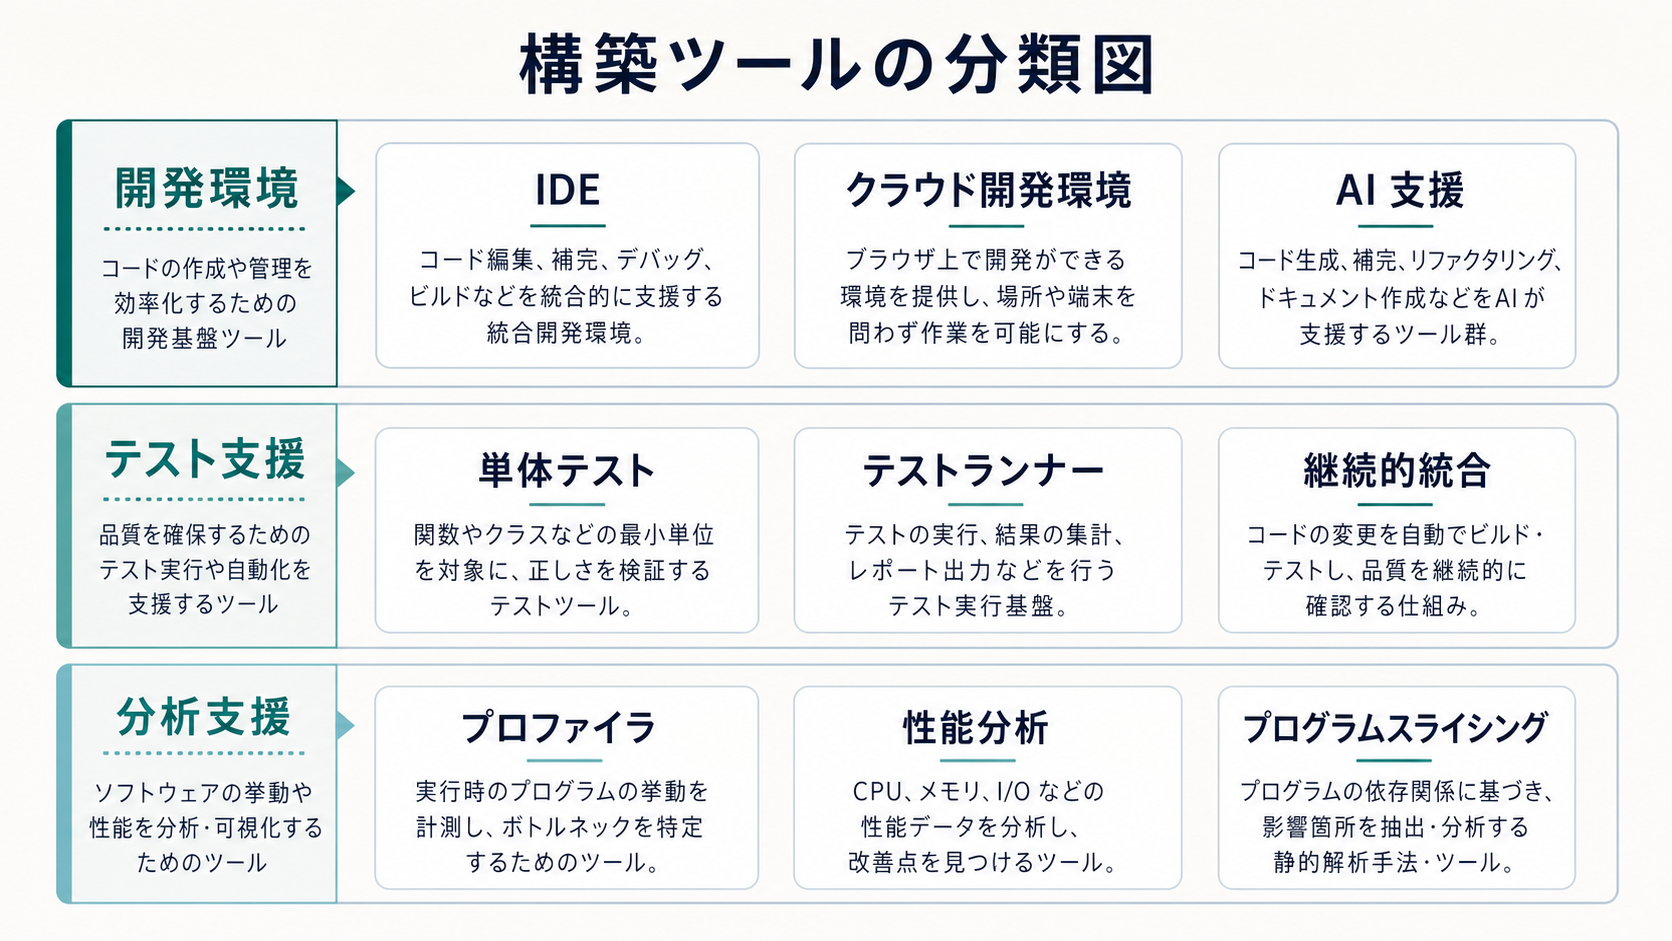
\includegraphics[width=0.96\linewidth]{assets/fig-ch04-15.png}}{\fbox{\parbox[c][48mm][c]{0.9\linewidth}{\centering 画像生成待ち\\構築ツールの分類図}}}
\caption{構築ツールの分類図}
\label{fig:ch04-15}
\end{figure}
